% !TeX spellcheck = en_GB
%\begin{landscape}
\begin{figure}[h]
	\centering
	% 21/12
	\begin{subfigure}[b]{0.8\textwidth}
		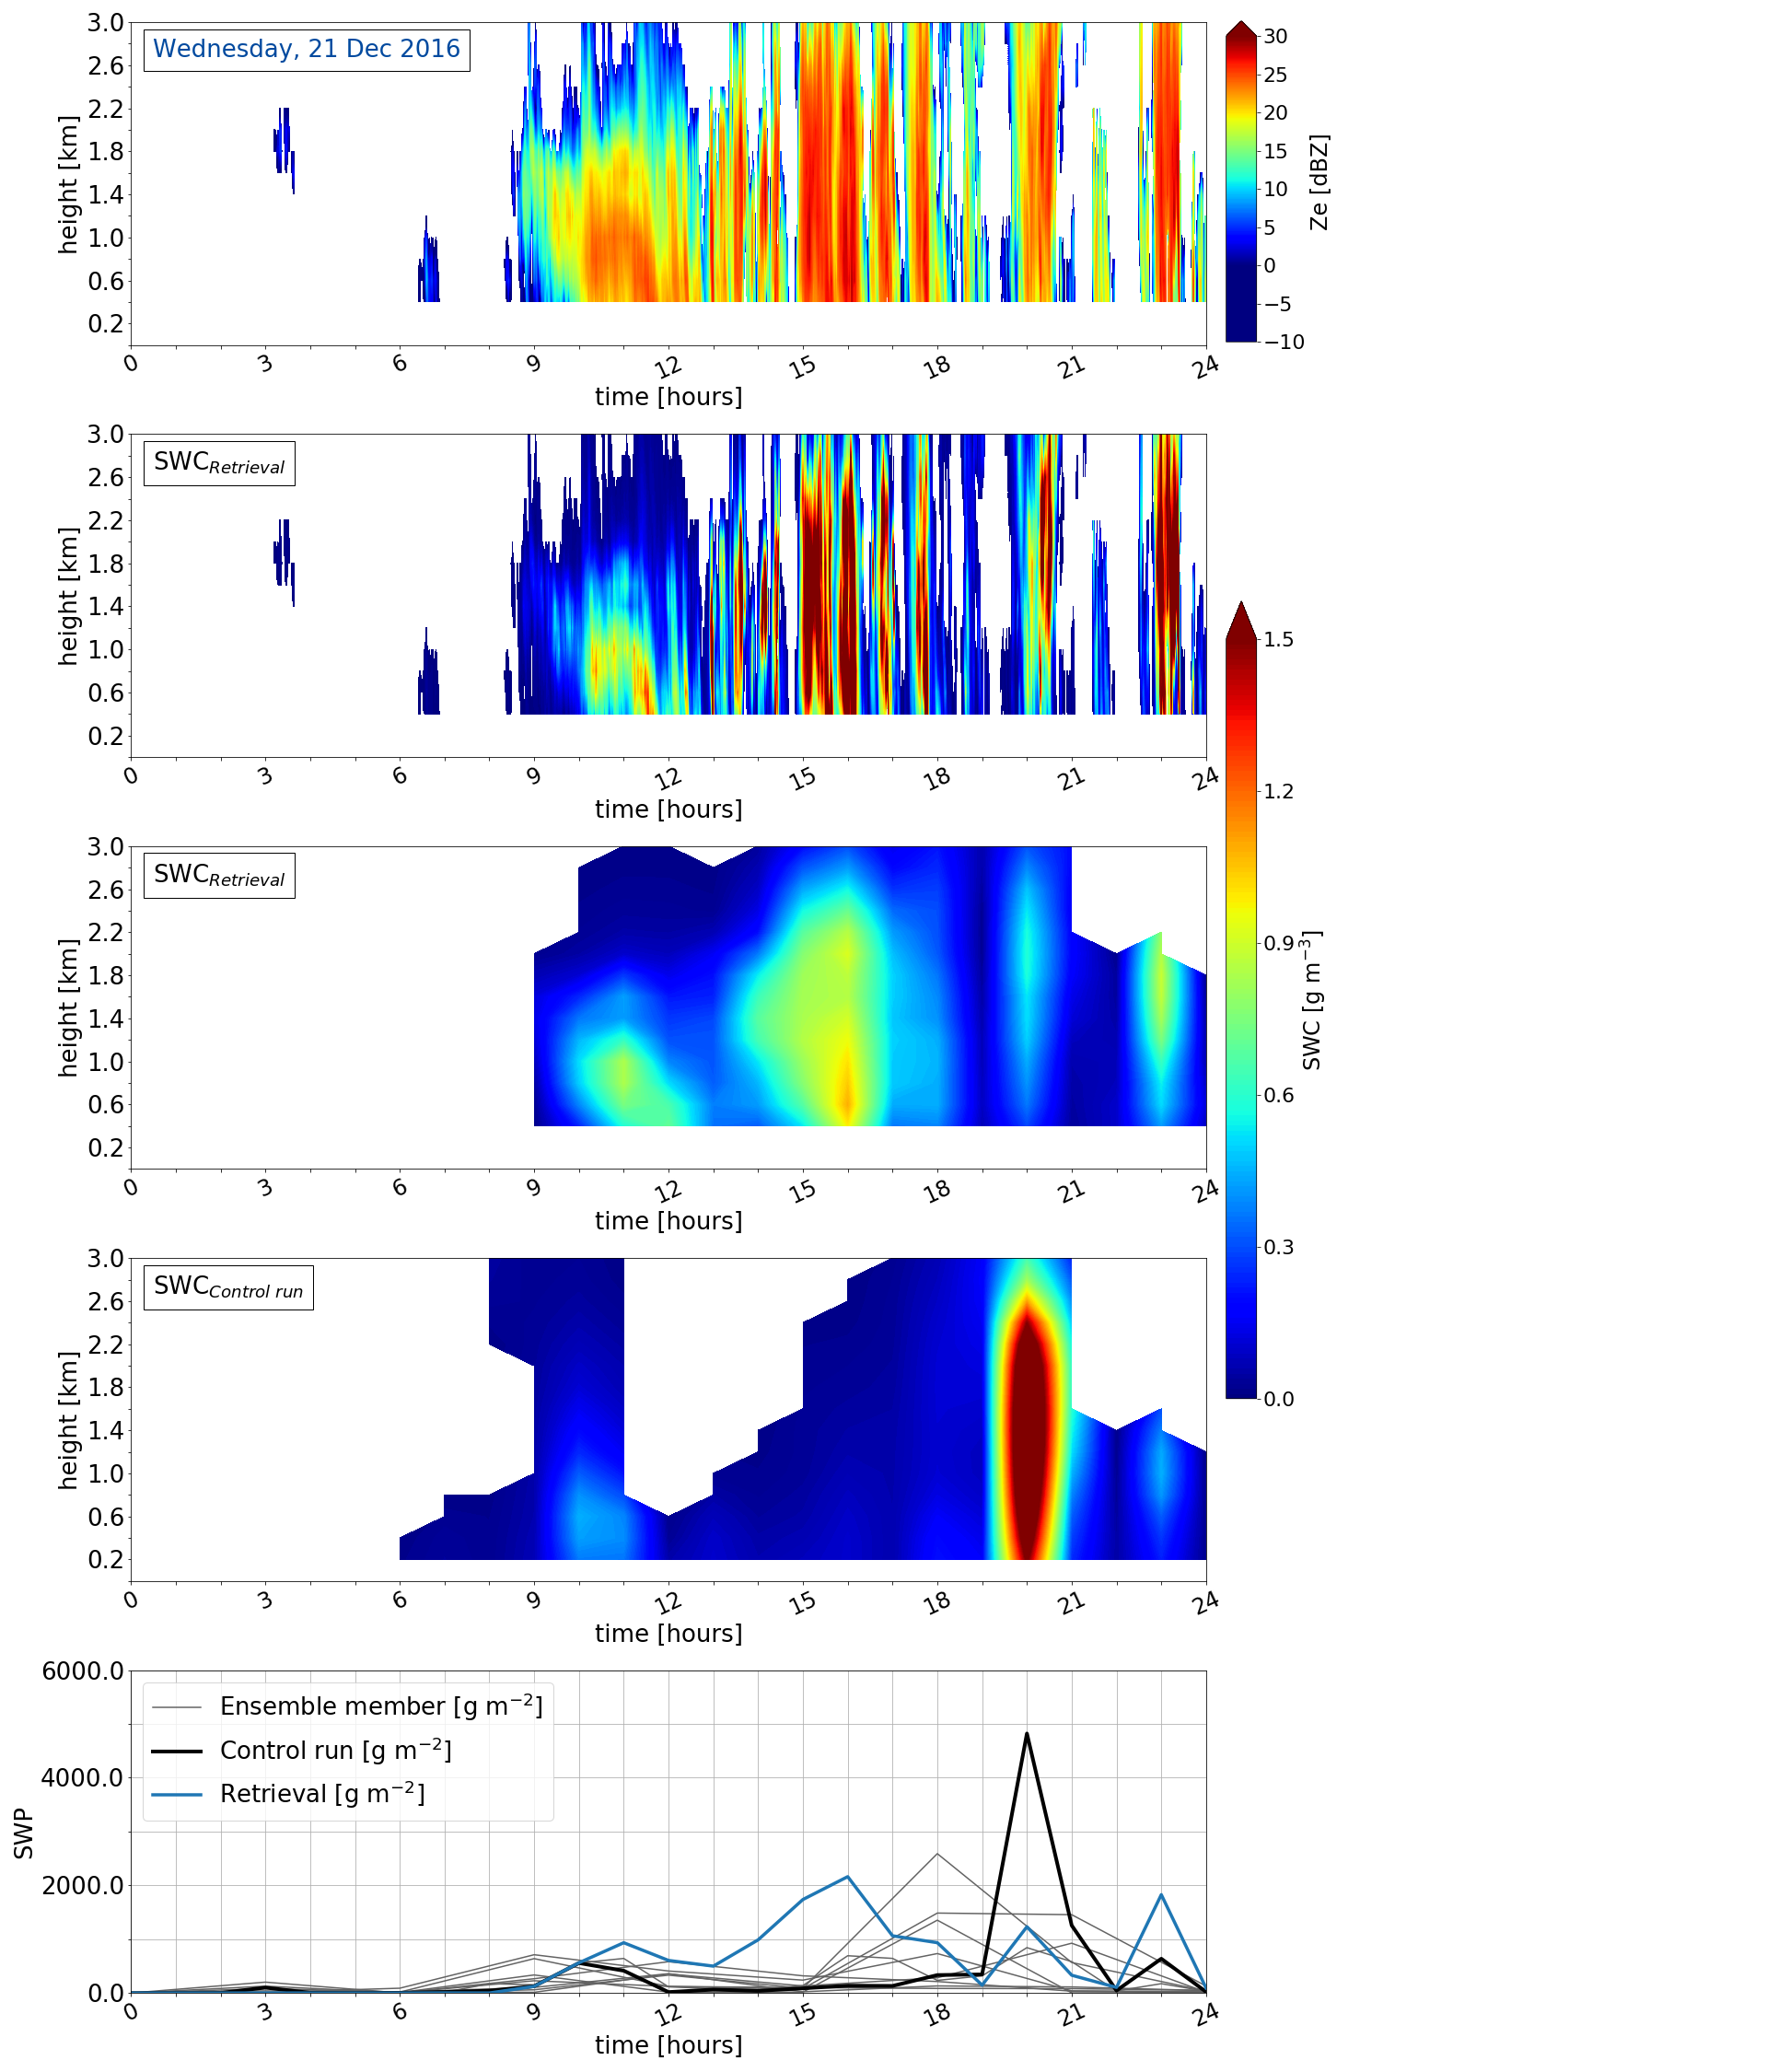
\includegraphics[trim={0.5cm 0.5cm 17.5cm .5cm},clip,width=\textwidth]{./fig_SWC/20161221}
		\caption{Wednesday, \SI{21}{\dec}}\label{fig:SWC21}
	\end{subfigure}
\end{figure}
\begin{figure}\ContinuedFloat
	\centering
	% 22/12
	\begin{subfigure}[b]{0.8\textwidth}
		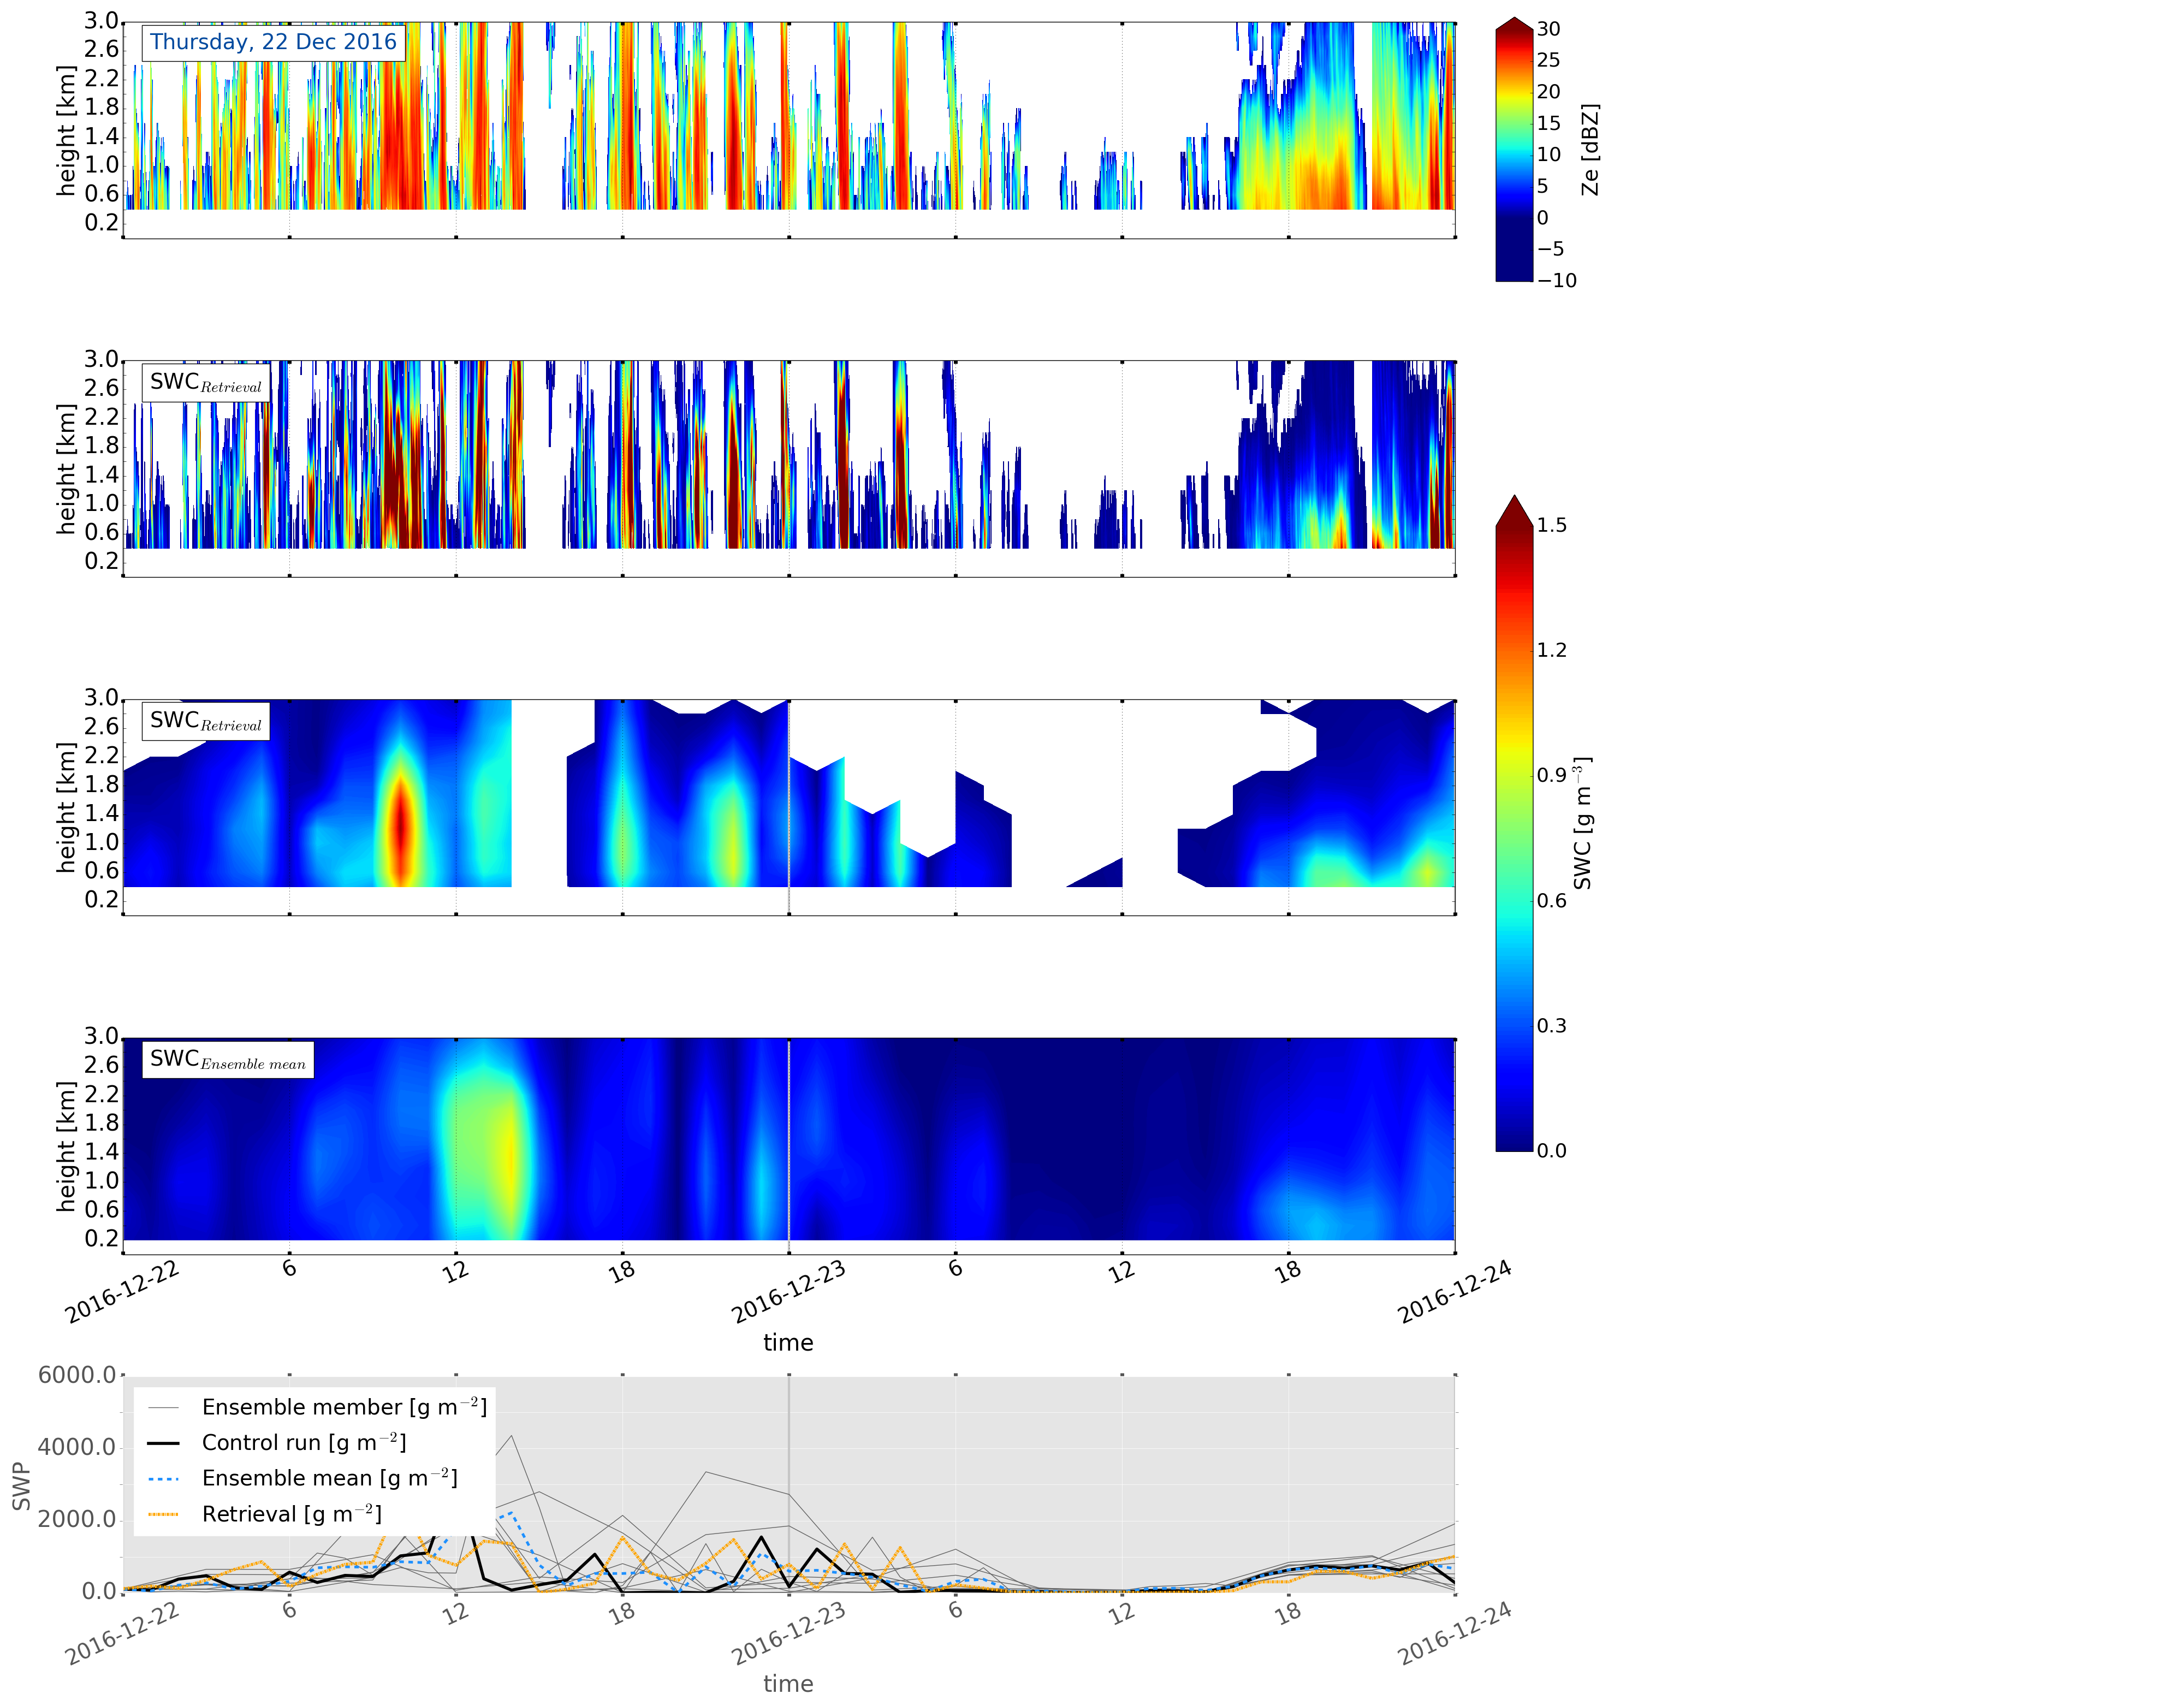
\includegraphics[trim={0.5cm 0.5cm 17.5cm .5cm},clip,width=\textwidth]{./fig_SWC/20161222}
		\caption{Thursday, \SI{22}{\dec}}\label{fig:SWC22}
	\end{subfigure}
\end{figure}
\begin{figure}\ContinuedFloat
	\centering
	% 23/12
	\begin{subfigure}[b]{0.8\textwidth}
		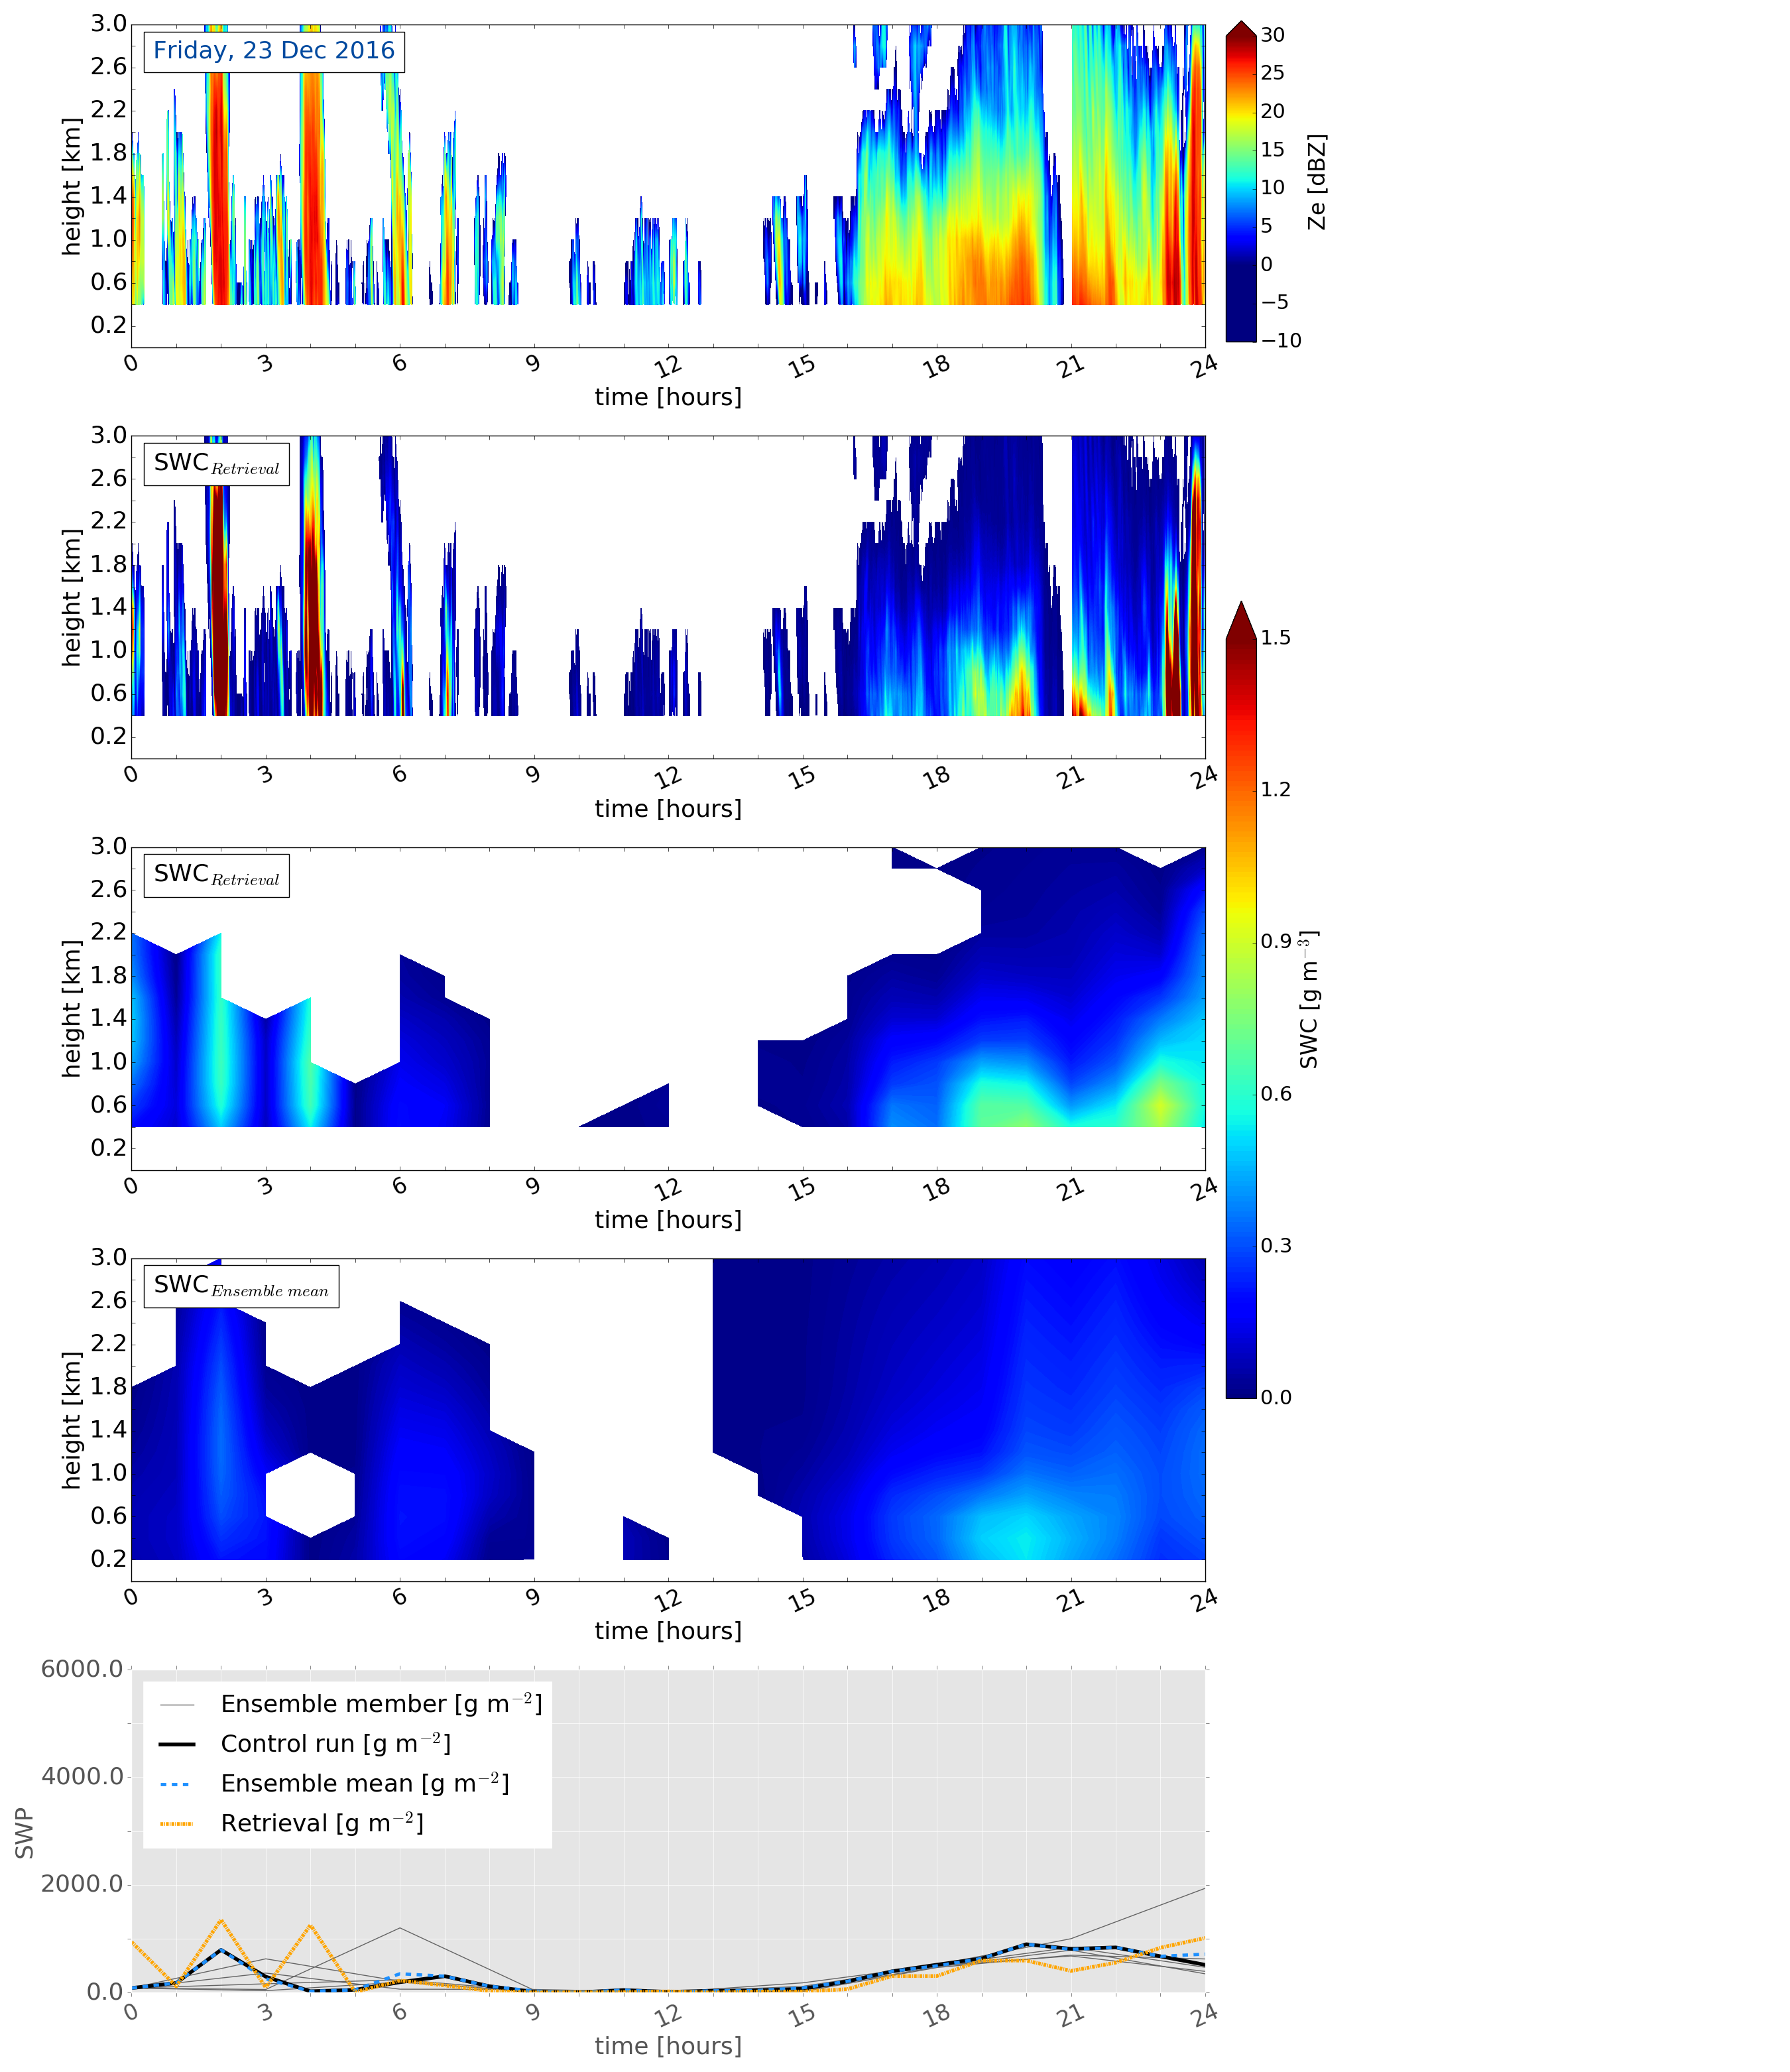
\includegraphics[trim={0.5cm 0.5cm 17.5cm .5cm},clip,width=\textwidth]{./fig_SWC/20161223}
		\caption{Friday, \SI{23}{\dec}}\label{fig:SWC23}
	\end{subfigure}
\end{figure}
\begin{figure}\ContinuedFloat
	\centering
	% 24/12
	\begin{subfigure}[b]{0.8\textwidth}
		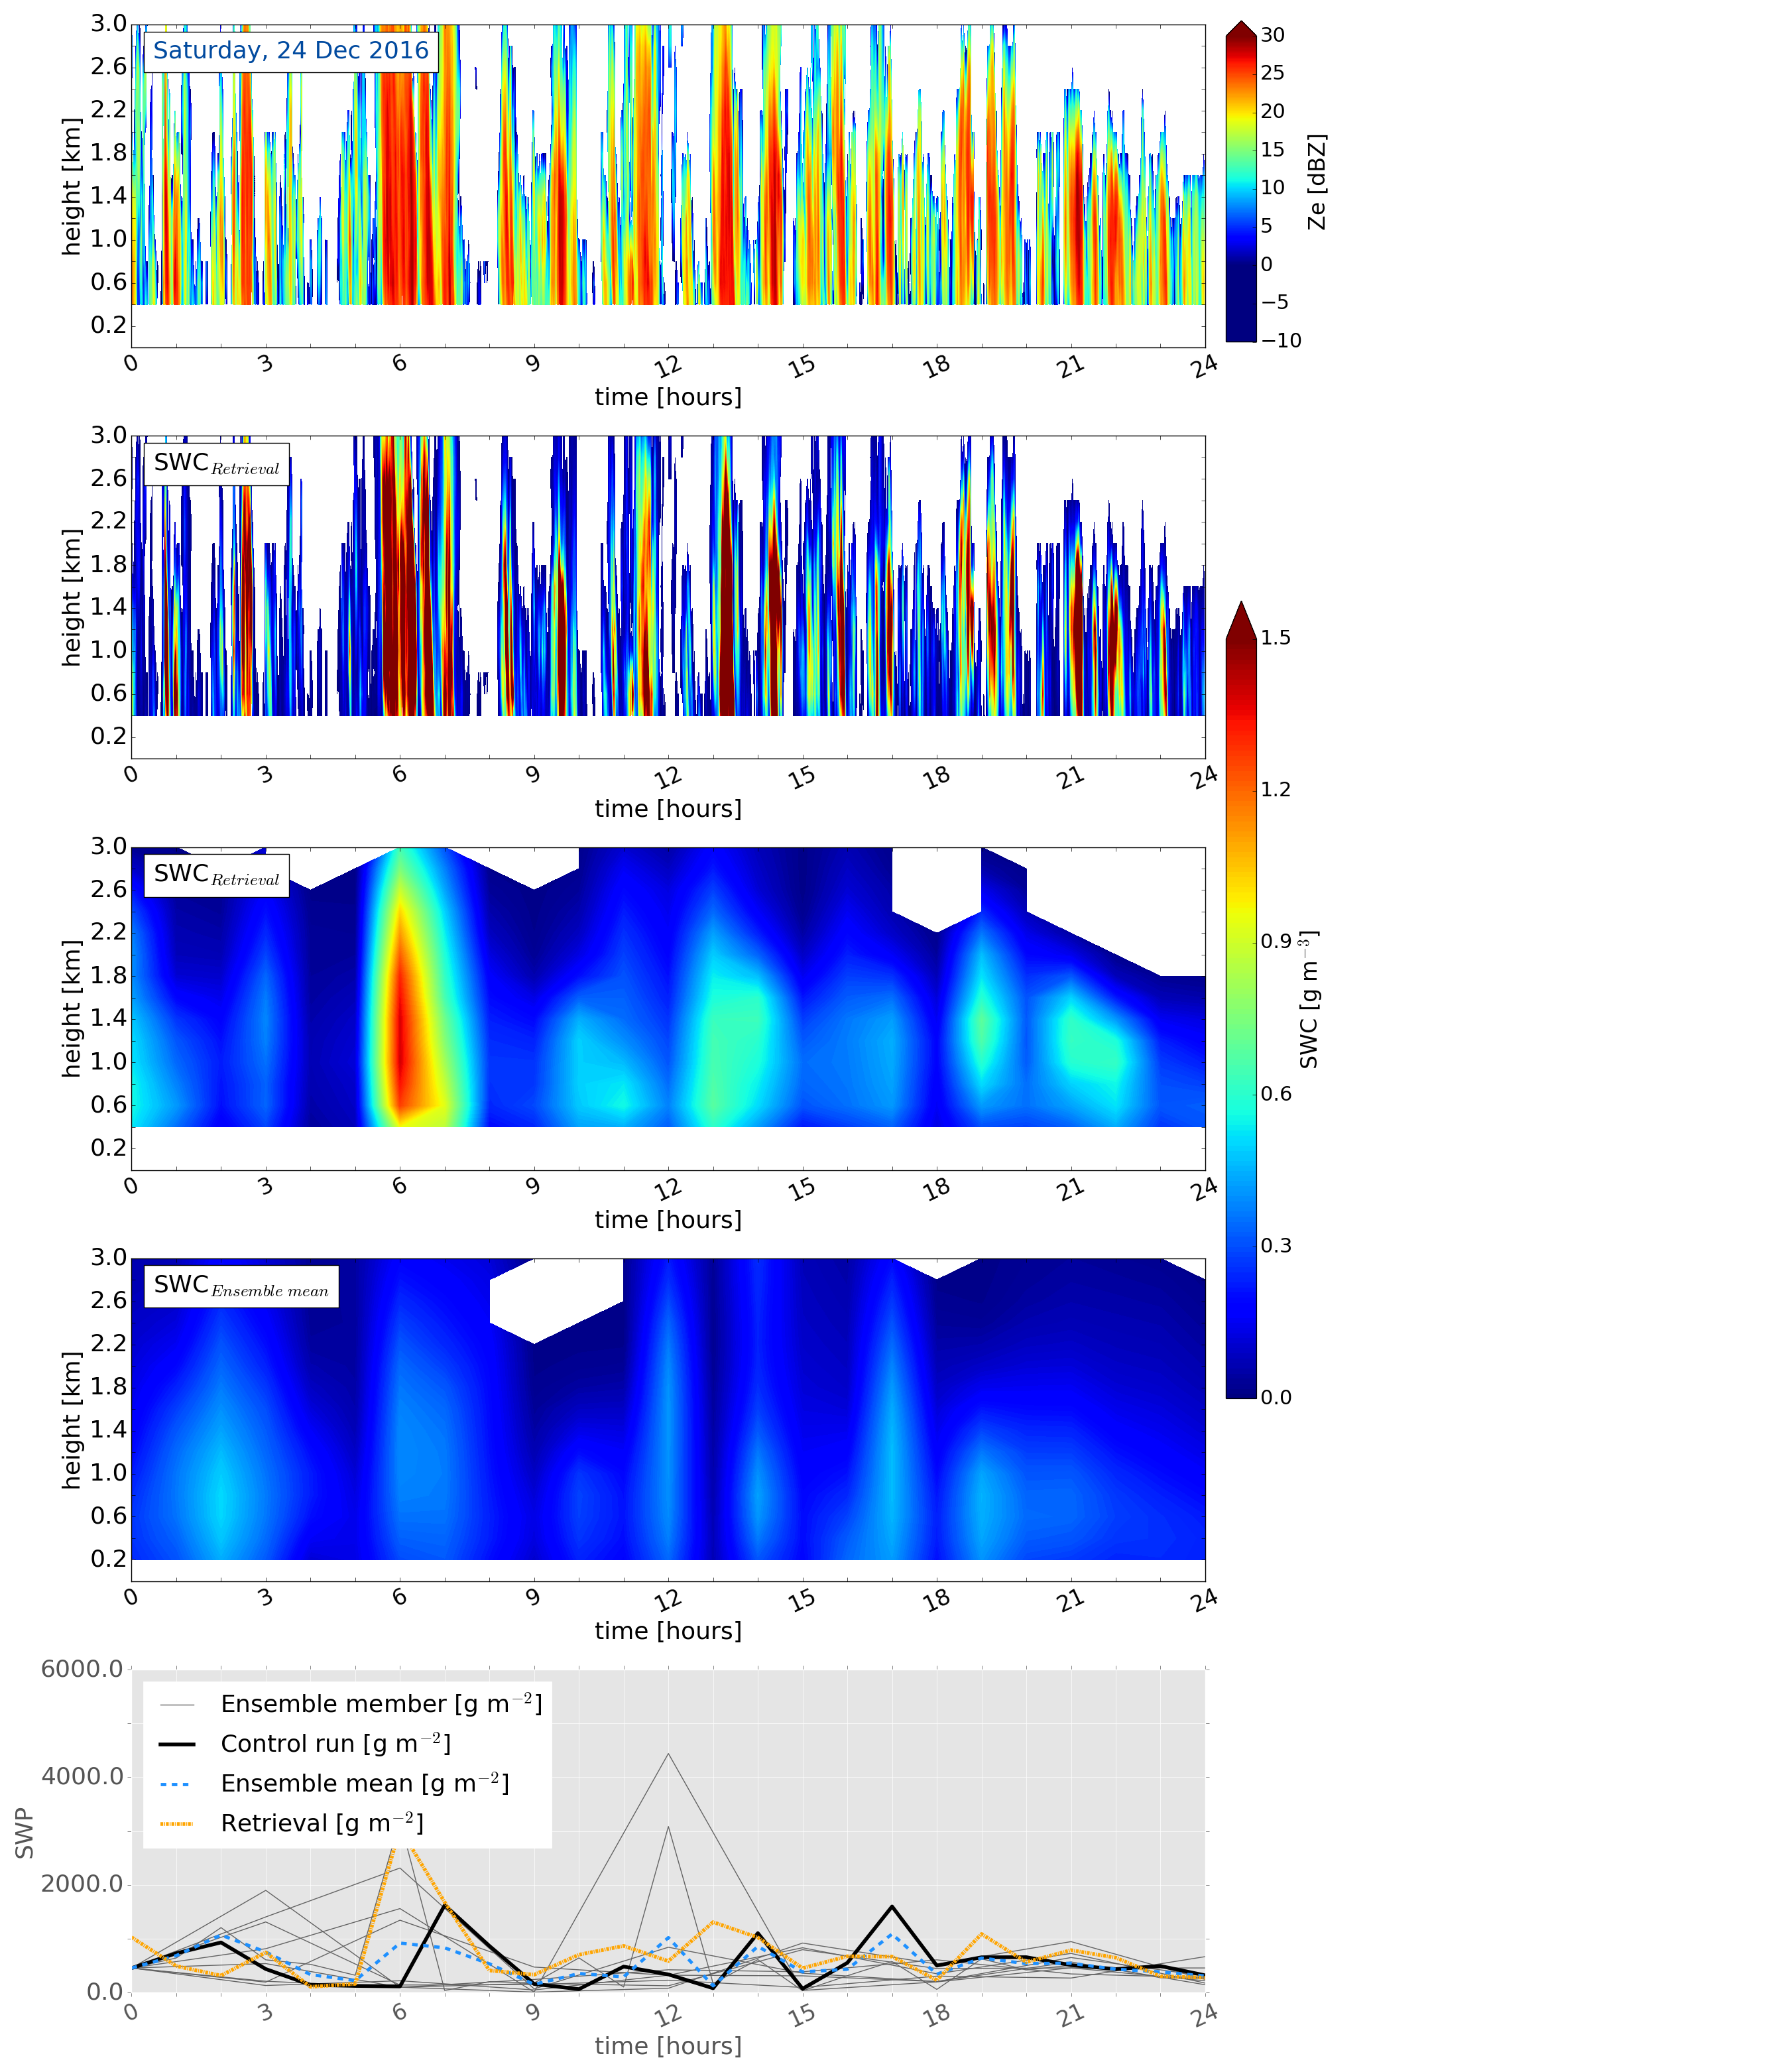
\includegraphics[trim={0.5cm 0.5cm 17.5cm .5cm},clip,width=\textwidth]{./fig_SWC/20161224}
		\caption{Saturday, \SI{24}{\dec}}\label{fig:SWC24}
	\end{subfigure}
\end{figure}
\begin{figure}\ContinuedFloat
	\centering
	% 25/12
	\begin{subfigure}[b]{0.8\textwidth}
		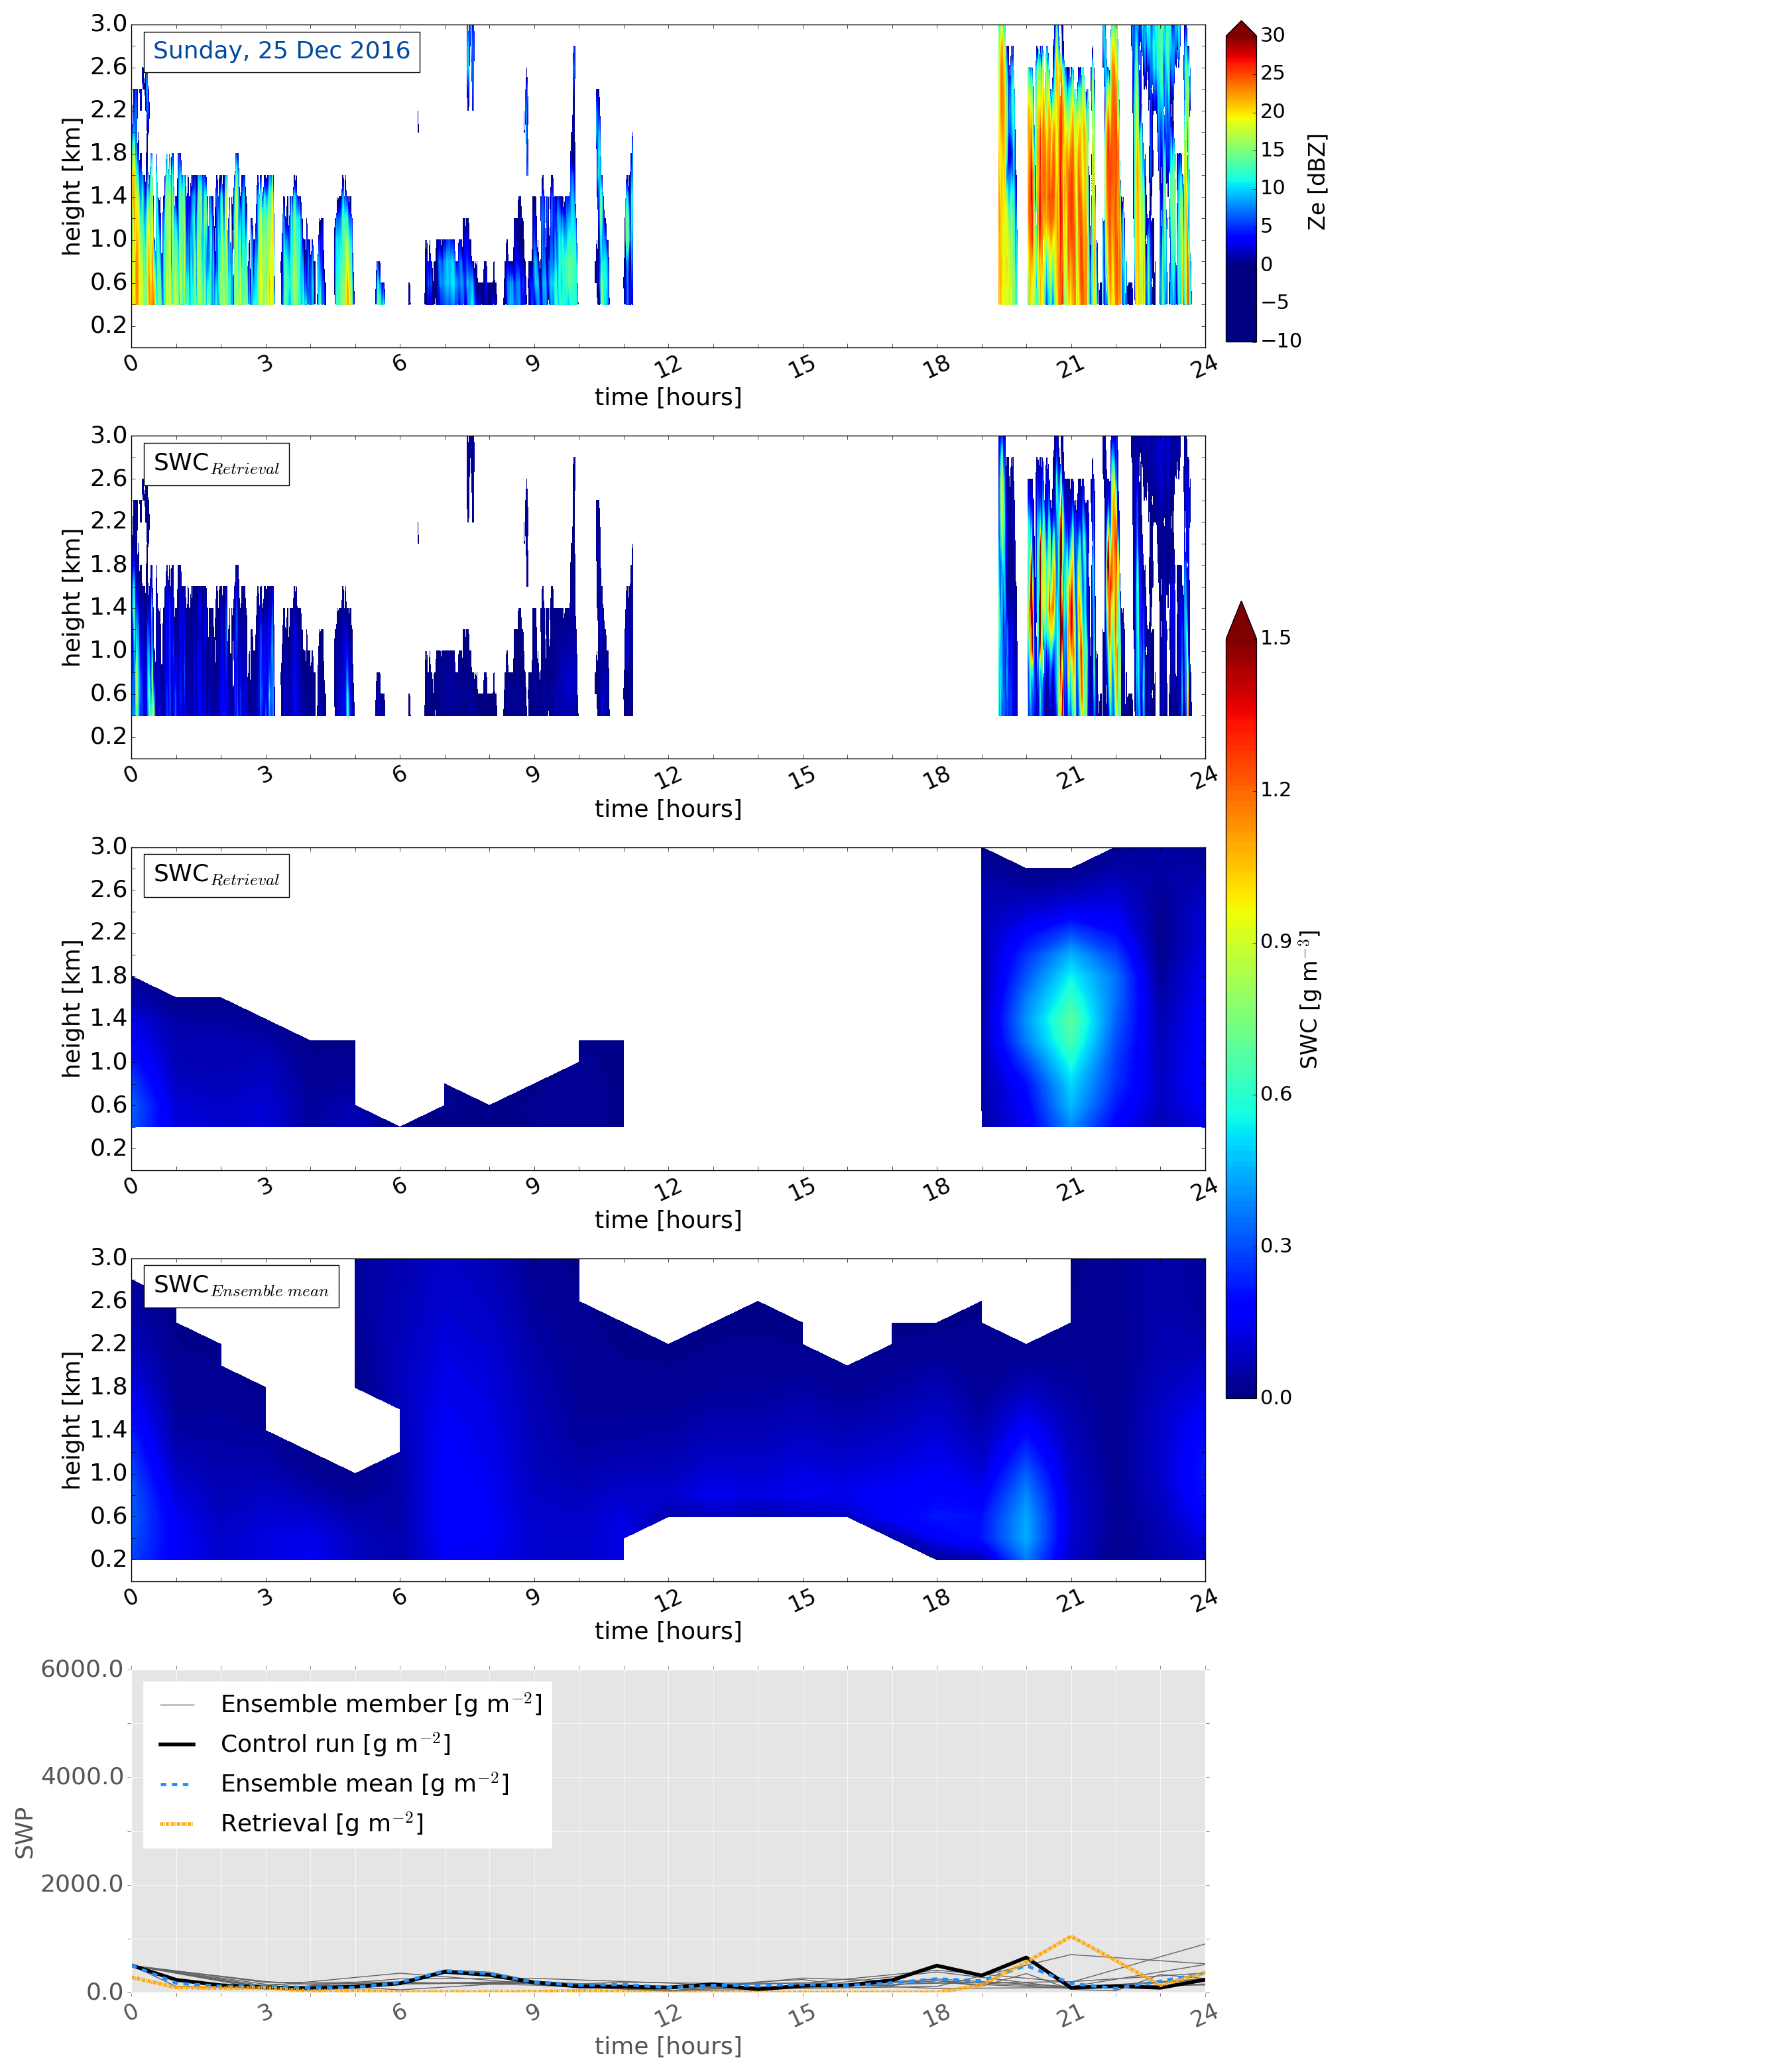
\includegraphics[trim={0.5cm 0.5cm 17.5cm .5cm},clip,width=\textwidth]{./fig_SWC/20161225}
		\caption{Sunday, \SI{25}{\dec}}\label{fig:SWC25}
	\end{subfigure}
\end{figure}
\begin{figure}\ContinuedFloat
	\centering
	% 26/12
	\begin{subfigure}[b]{0.8\textwidth}
		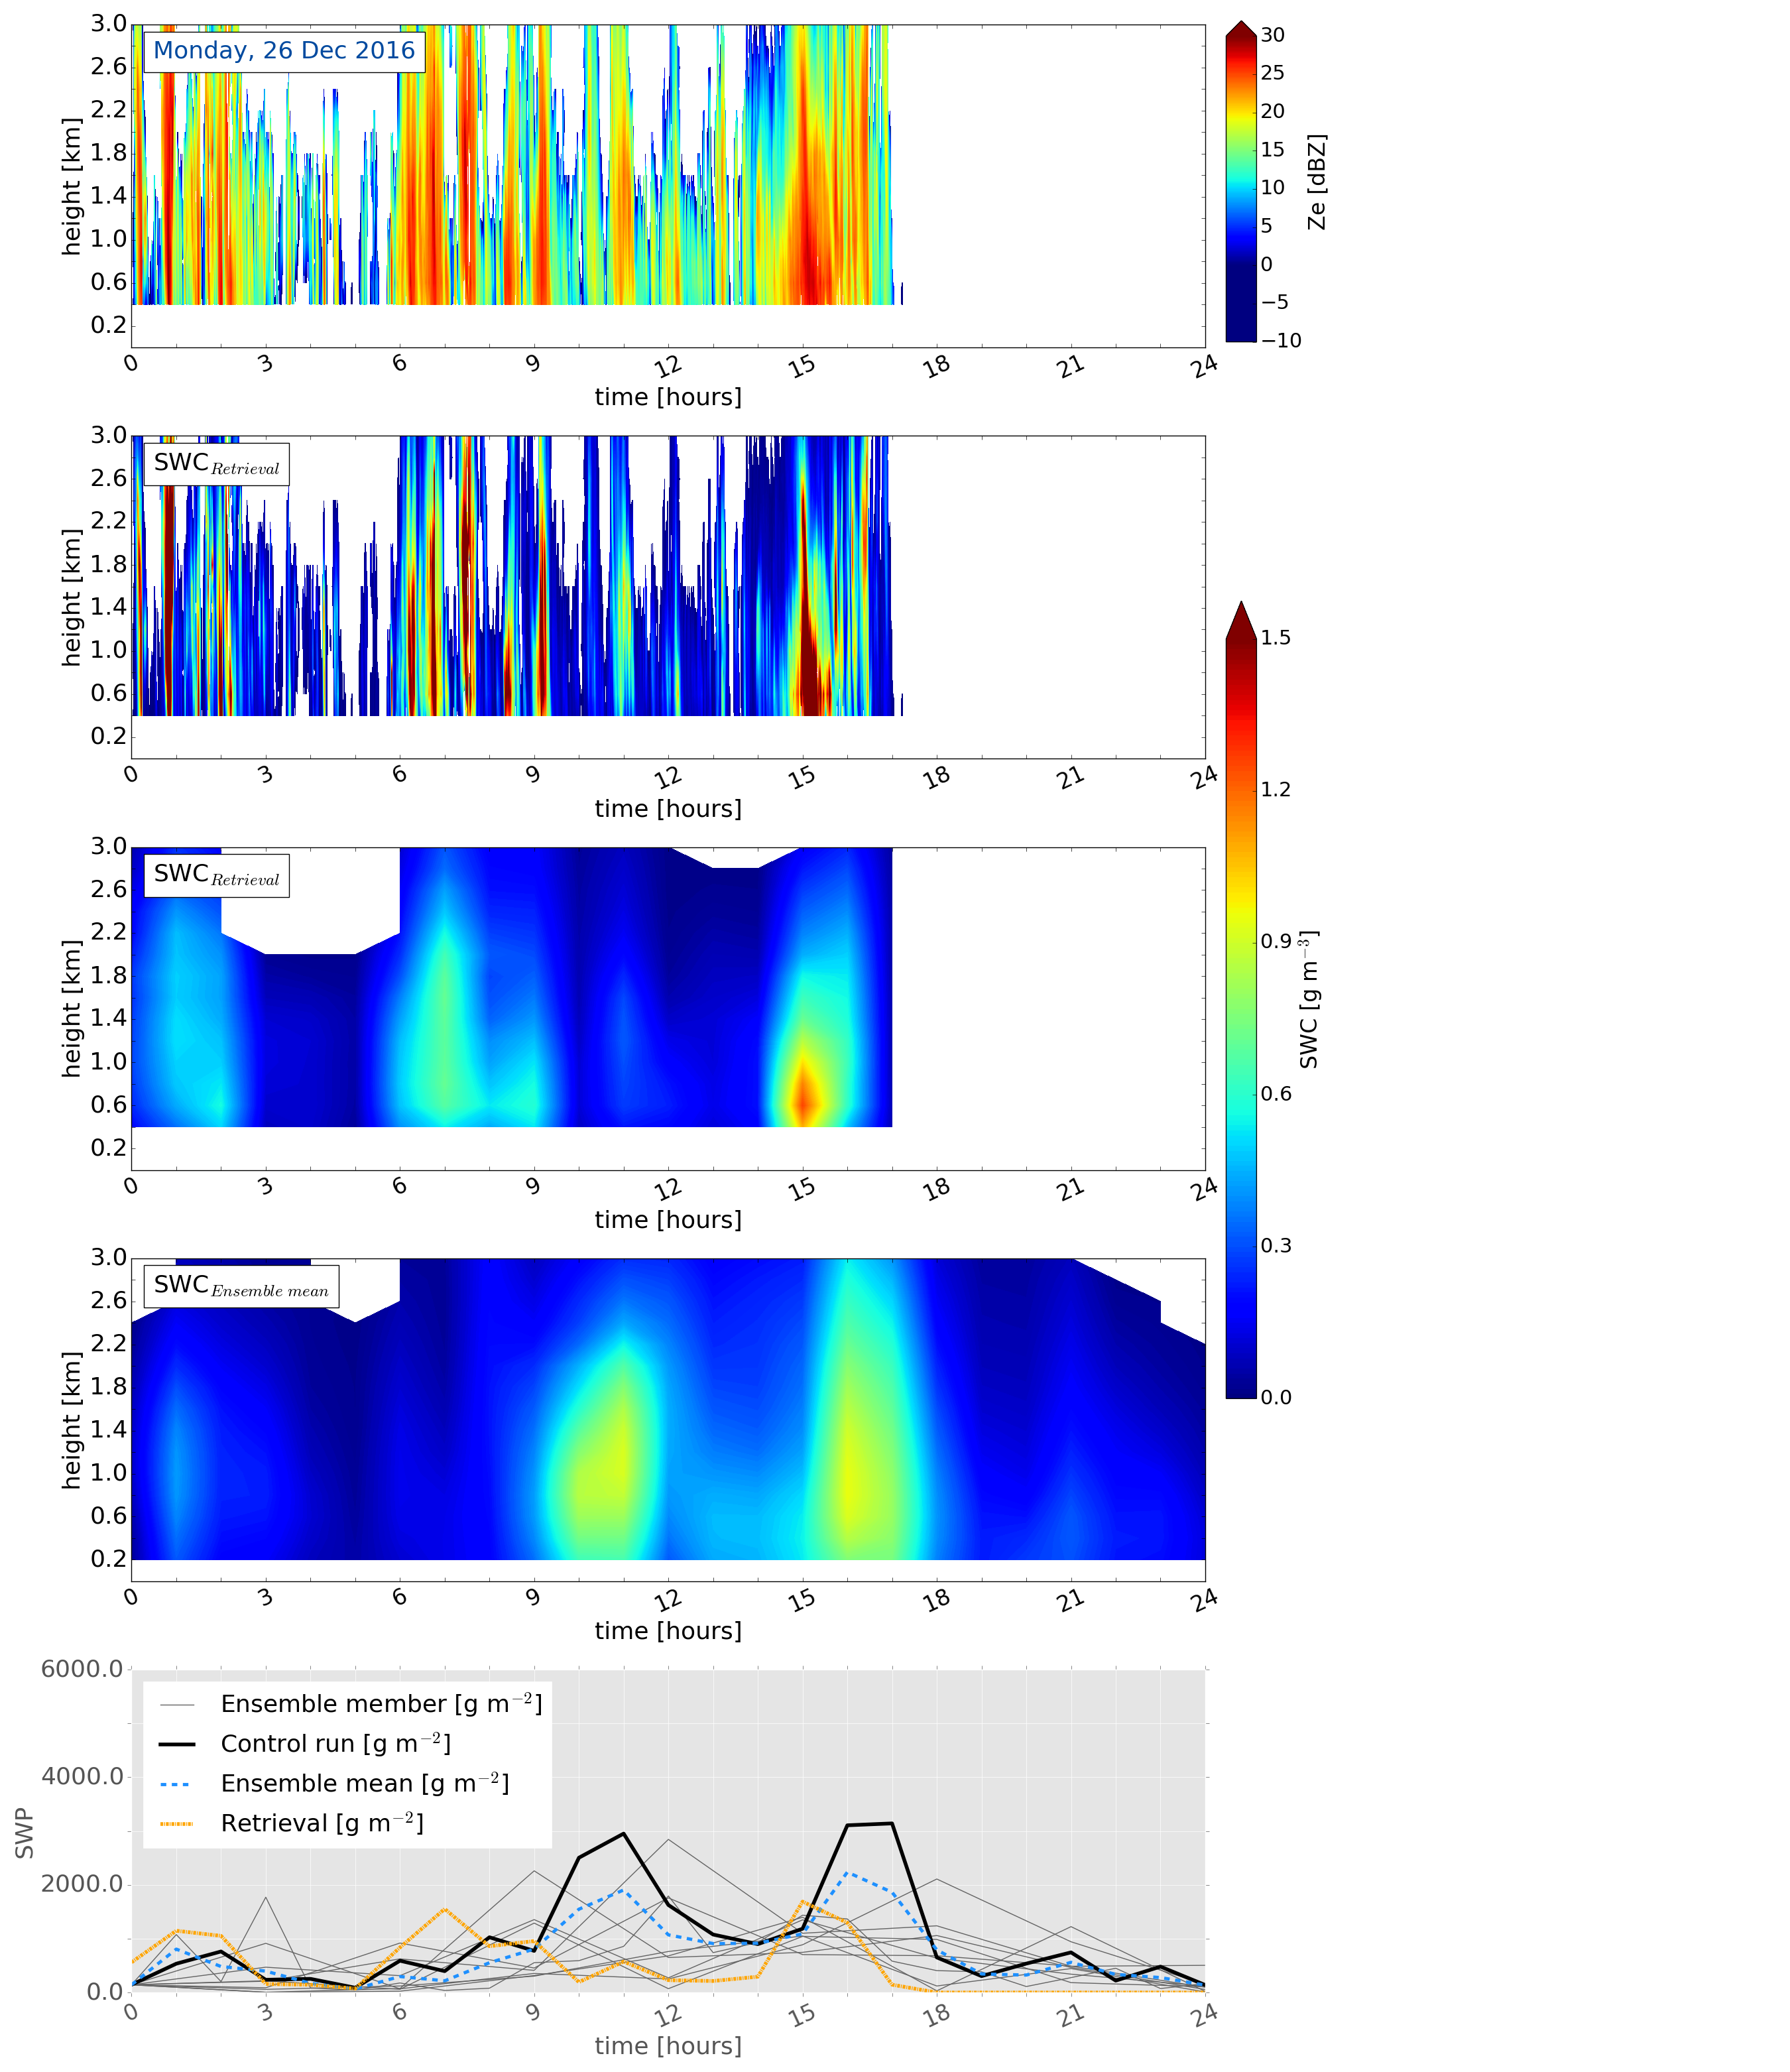
\includegraphics[trim={0.5cm 0.5cm 17.5cm .5cm},clip,width=\textwidth]{./fig_SWC/20161226}
		\caption{Monday, \SI{26}{\dec}}\label{fig:SWC26}
	\end{subfigure}
	\caption{Upper panel: MRR reflectivity in \SI{}{\dB Z}. 2nd panel: SWC optimal estimation retrieval output every second in \SI{}{\SWC}. 3rd panel: hourly-averaged SWC optimal estimation retrieval output. 4th panel: \SI{200}{\metre}-averaged SWC ensemble mean forecast from MEPS. Lowest panel: SWP from MEPS, initialised at \SI{00}{\UTC}. Black line represents the deterministic forecast, the doted orange line the ensemble mean and the grey lines the nine perturbed members. In red the SWP from the averaged retrieval output.}\label{fig:SWC}
\end{figure}

